\documentclass[12pt]{article}
\usepackage[papersize={8cm,12cm},margin={.5cm,.5cm}]{geometry}
\usepackage{common}
\usepackage{graphicx}
\usepackage{amssymb}
\makeatletter
\DeclareFontFamily{U}{tipa}{}
\DeclareFontShape{U}{tipa}{m}{n}{<->tipa10}{}
\newcommand{\arc@char}{{\usefont{U}{tipa}{m}{n}\symbol{62}}}%
\newcommand{\arc}[1]{\mathpalette\arc@arc{#1}}
\newcommand{\arc@arc}[2]{\sbox0{$\m@th#1#2$}%
  \vbox{
    \hbox{\resizebox{\wd0}{\height}{\arc@char}}
    \nointerlineskip
    \box0
  }%
}
\makeatother
\newcommand{\slantparallel}{\mathrel{\mkern-2mu/\mkern-4mu/\mkern-2mu}}
\begin{document}
\begin{problem}
\item[8.] 梯形 $ABCD$ 中,$\overline{AD} \slantparallel \overline{BC}$,且有一圓 $O$ 通過 $A$、$B$、$C$ 三點,使 $\overline{AD}$ 與圓 $O$ 相切於 $A$ 點,如圖(八)所示。若 $\angle B = 58^\circ$,則 $\arc{BC}$ 的度數為何?
  \begin{figure}[ht]
    \centering
    \vspace*{-1ex}
    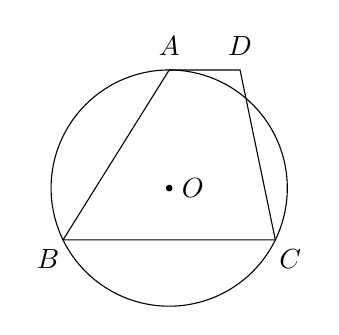
\begin{tikzpicture}
      \filldraw (0,0) circle (1pt);
      \draw (0,0) circle (1.5cm);
      \draw (0,1.5) -- (-1.348,-.658) -- (1.348,-.658) -- (.9,1.5) -- (0,1.5);
      \node at (.3,0) {$O$};
      \node at (0,1.8) {$A$};
      \node at (-1.538,-.898) {$B$};
      \node at (1.538,-.898) {$C$};
      \node at (.9,1.8) {$D$};
    \end{tikzpicture}
    \vspace*{-1ex}
    \caption*{圖(八)}
    \vspace*{-2ex}
  \end{figure}
  \begin{choices}
    \item 116
    \item 120
    \item 122
    \item 128
  \end{choices}
\end{problem}
\end{document}
